\subsection{lettuce}

\begin{frame}
\begin{center}
\huge{lettuce}

\bigskip

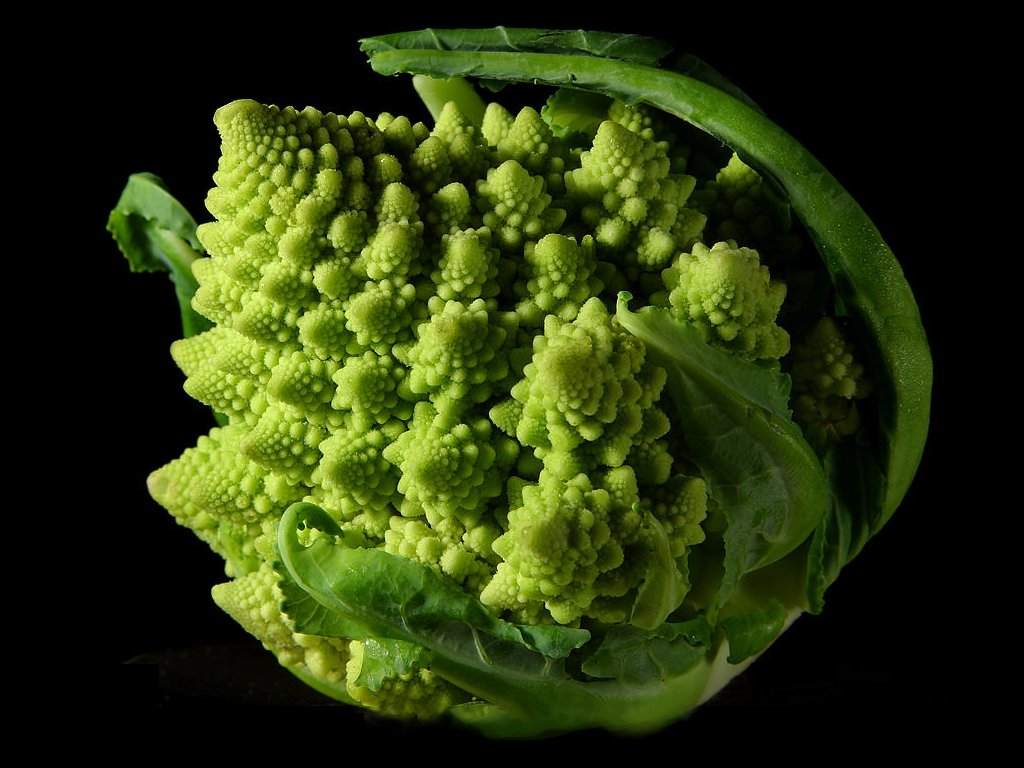
\includegraphics[width=7cm,height=7cm]{images/lettuce.jpg}
\end{center}
\end{frame}

\begin{frame}[fragile]
\begin{minted}{cucumber}
Feature: Compute factorial
    In order to play with Lettuce
    As beginners
    We'll implement factorial

    Scenario: Factorial of 0
        Given I have the number 0
        When I compute its factorial
        Then I see the number 1
\end{minted}
\end{frame}

\begin{frame}[fragile]
\begin{minted}{python}
from lettuce import *

@step('I have the number (\d+)')
def have_the_number(step, number):
    world.number = int(number)

@step('I compute its factorial')
def compute_its_factorial(step):
    world.number = factorial(world.number)

@step('I see the number (\d+)')
def check_number(step, expected):
    expected = int(expected)
    assert world.number == expected, \
        "Got %d" % world.number

def factorial(number):
    return -1
\end{minted}
\end{frame}

\begin{frame}
\begin{itemize}
\item Inspirováno {\bf Ruby} knihovnou {\tt Cucumber}
\item Test je popsán v čistém textu
\item Musí se definovat parsery jednotlivých kroků
\end{itemize}
\end{frame}
